\startfirstchapter{Introduction}
\label{chapter:introduction}


In this thesis, we consider solving linear inverse problems using nonconvex l p and TV p
regularizers with 0 < p < 1, and applications of the proposed optimization models in
the general area of signal recovery including signal denoising and compressive sensing
of 1-D signals and 2-D images. 

The purpose of this chapter is to introduce the
literature relevant to the problems considered, discuss the motivations for improving
the existing methods, and describe the main contributions and structure of the thesis.

\section{The Localization Problem: Motivation} \label{problem}

Geolocation is a rapidly growing field due to the large impact it has on daily life.  The general public has become increasingly dependent on it for realtime navigation, particularly on mobile smartphone devices. Location-based services are  playing an increasingly important role in other fields such as teleconferencing, wireless communications, surveillance, and geophysics \cite{SmithAbel, ShcauRob, Yao, Huang, CheungChan, LiHu, Cheung, Sayed, classMDS}.

Different technologies have been used to build geolocation systems. Several global navigation satellite systems that are available for both military and civilian use and include GPS(US), Galileo(EU), GLONASS(Russia), BeiDou(China). Satellites are equiped with atomic clocks that provide a high-accuracy timing signal to  allow a receiver to calculate the time that it takes the signal to reach the receiver. This information is used to calculate the position of the receiver by using a a computational technique known as trilateration. The location of the receiver can be calculated from the
tracked positions of the satellites and the times measured, each known as the Time-of-Arrival (TOA) \cite{GeoLoc}.

%Consequently, it
%has been incorporated into many services and applications. Currently, outdoor
%localization, thanks to GPS, has revolutionized navigation-based applications running on automotive GPS-enabled devices and smart phones. Applications range from location awareness, to point-by-point directions between destinations, to identifying the closest cinema or coffee shop. The success of GPS has been due to the reliability, availability, and practical accuracy that the system can deliver; however, GPS lacks coverage indoors and in urban areas, in particular near buildings when the signal is blocked;
%even in the best of conditions, the accuracy is on the order of several meters. 
%navigation:
%auto
%aerial
%ships and boats
%heavy equipment
%fitness trackers (for example, Garmin gps enabled smart watches for tracking the run distance/routes/speed)

As localization technologies become more accurate and robust, location services are becoming increasingly integrated into daily life.
GPS was the first to be developed and made available to the public. Therefore it has been used as the basis of many services and applications.
In particular it has revolutionized navigation-based applications running on smartphones and in automobiles. Use cases include point-by-point directions between destinations and identifying nearby facilities or points of interest (such as the closest coffee shop).
GPS is also widely used in navigation of other vehicles such as airplanes, ships, and heavy equipment. It has also been used for monitoring movements rather than navigating, for example in fitness trackers such as FitBit \cite{FB} and Garmin\cite{Garmin} which automatically collect data about the user's activities (distance run, speed, routes taken).

The widespread adoption and success of GPS in these different application domains is due to its accuracy, reliability and availability. However, there are still limitations to be overcome. GPS coverage is limited indoors and in urban areas due to buildings obstructing the signals between the GPS device and satellites. Additionally, the accuracy is on the order of several meters. While this is sufficient for many applications such as navigating to the nearest coffee shop, greater accuracy will open up new opportunities, particularly for indoor positioning where spaces are smaller and greater precision is required.

%The integration of location services into our day-to-day life will grow significantly
%over the next decade as technologies mature and accuracy improves. 
%Development of localization technologies has been occurring independently for different wireless systems.
%The Global Positioning System (GPS) was the first to be developed and made available to the public. Therefore it has been used as the basis of many services and applications.
%The evolution
%of localization technologies has occurred independently for different wireless sys-
%tems/standards. The Global Positioning System (GPS) was the first system to bring
%to light the benefits of accurate and reliable location information. Consequently, it
%has been incorporated into many services and applications. 
%Currently, outdoor
%localization, thanks to GPS, has revolutionized navigation-based applications
%running on automotive GPS-enabled devices and smart phones. Applications range
%from location awareness, to point-by-point directions between destinations, to
%identifying the closest cinema or coffee shop. 
%The basic technology behind the
%system is to measure the time elapsed for a signal to travel between a number of
%satellites orbiting the globe and a mobile device. 
%Through a computational tech-
%nique known as triangulation, the location of the mobile can be calculated from the
%tracked positions of the satellites and the times measured, each known as the Time-
%of-Arrival. The success of GPS has been due to the reliability, availability, and
%practical accuracy that the system can deliver; however, GPS lacks coverage
%indoors and in urban areas, in particular near buildings when the signal is blocked;
%even in the best of conditions, the accuracy is on the order of several meters.

As a result there has been a desire for new location-based services with improved accuracy and coverage. One of the approaches to the problem was integration of various wireless technologies with GPS. One such solution is called Assisted GPS (A-GPS), which distributes data and processing over a network of cellular towers equipped with GPS-enabled servers \cite{AGPS}. This can greatly reduce the search space and time to first fix on location. Other systems were built purely on cellular signals, adapting the TOA techniques originally developed for GPS. However their accuracy was limited in urban environments due to obstruction of signals by buildings, and the technique did not gain widespread use beyond the Emergency-911 system it was developed for in the United States.

% Paper: http://www.cs.columbia.edu/~drexel/CandExam/Geolocation_assistedGPS.pdf

%utilizes cellular networks to provide devices with information about which are the closest GPS satellites. This allows the GPS device to determine its position more quickly \cite{Richton, 2001}. The burden of the computationally expensive triangulation calculations can also be offloaded from the mobile device to base stations which do the computation and return the position information to the mobile device. This can significantly improve performance on CPU-constrained devices.

%As the growth of the number of smart devices and mobile users continues to
%increase without bound, the desire for new location-based services that require
%enhanced accuracy, including in GPS-denied areas, has emerged. To address this
%challenge, novel solutions attempt to integrate different wireless technologies with
%GPS. For example, assisted GPS (A-GPS) was developed to provide better locali-
%zation information in limited coverage areas by decreasing the time necessary for
%GPS to obtain a position fix (Richton 2001). Specifically, in A-GPS, cellular
%
%networks furnish GPS-equipped mobile devices with satellite constellation infor-
%mation such that they can identify the closest orbiting satellites a priori, providing a
%faster lock. In addition, A-GPS relieves the burden of the computationally intensive
%triangulation technique from the CPU-limited mobile device by forwarding the links
%the GPS receiver measures to the base stations (BSs), which then calculate the
%mobile’s position and return the information to the mobile device.



With the proliferation of smartphone devices and the internet,
WiFi access points are becoming increasingly widespread, 
providing another means of determining location. One type of WiFi-based technique is called Received Signal Strength (RSS) location fingerprinting. It uses a database of WiFi signatures (RSS values and MAC address) along with GPS coordinates. This has to be built up ahead of time, for example by surveying a city with a GPS and WiFi enabled vehicle. Realtime location of a device is determined by finding the best match between RSS values detected by the mobile device, and those stored in the database. Accuracy in the range of tens of meters can be achieved in urban areas where wireless access points are plentiful. A company called Skyhook Wireless developed one such system. \cite{Skyhook}


%Unsurprisingly, the next logical evolution of localization systems emerged from
%the cellular domain, where the requirement for localization was spearheaded by the
%Emergency-911 (E-911) mandate. Before GPS was widely available on mobile
%phones, cellular operators adopted and deployed varying technologies to locate
%mobiles within a cell radius. Time-Of-Arrival-based computational techniques,
%which originated from GPS systems, were adapted in order to achieve similar
%localization performance for the common cell phone channel sharing (multiplex-
%ing) schemes: Time Division Multiple Access (TDMA) and Code Division
%Multiple Access (CDMA). The use of cellular localization was limited to E-911
%due to the difficulty in achieving useful accuracy especially in urban environments.
%The poor accuracy stemmed from clusters of buildings in urban and suburban
%residential areas which brought about significant signal degradation due to mul-
%tipath and Non-Line-Of-Sight (NLOS) problems.
%At the same time, the popular IEEE 802.11 standard emerged, enabling ubiquitous deployment of Wi-Fi hotspots which sparked enthusiasm for an alternative
%to cellular localization. The rapid expansion of Wi-Fi access points (AP) across the
%urban/indoor environments made it possible for researchers to envision alterna-
%tives to TOA-based systems. Specifically, Received Signal Strength (RSS) location
%fingerprinting techniques emerged. One success story for deployment in the urban
%environment is Skyhook Wireless, a start-up company in the Boston area. Skyhook
%realized the potential of exploiting Wi-Fi signals emitted from residential homes
%and offices (available for free!) that are continuously in use—particularly in dense
%urban areas. Skyhook realized they could improve localization by building dat-
%abases of Wi-Fi signatures tied to locations that could be integrated to aid in the
%localization process. In essence, a survey is conducted by ‘‘wardriving’’ across a
%city with a Wi-Fi equipped device and a companion GPS receiver to record
%location. Wi-Fi RSS values and associated Medium Access Control (MAC) IDs
%are registered in a database for each location. During a localization query, a mobile
%device compares the RSSs measured from the registered APs to those in the
%database using a pattern matching technique. The mobile’s location is then
%determined by the best RSS match. Skyhook Wireless’s technology has attracted
%attention from the major players in the mobile device industry such as Apple and
%Google (Wortham 2009). The technique is very practical and delivers decent
%accuracy (tens of meters) for mobile location applications in outdoor urban
%environments where Wi-Fi APs are plentiful.
%Of course, the aforementioned triangulation fingerprinting techniques are not
%just applicable to GPS, cellular, or Wi-Fi networks. They can also be readily
%extended to virtually any pervasive radio-frequency source, in particular to tele-
%vision networks. In fact, the Rosum Corporation from Redwood City, CA took1.1 Overview
%3
%advantage of the 4.5 MHz of bandwidth available in broadcast TV channels.
%Besides the wide bandwidth available for accurate TOA estimation, the low carrier
%frequency offered excellent penetration through walls to mitigate NLOS condi-
%tions. The performance of different types of RF location systems in terms of cost
%and accuracy will vary widely. Other system design considerations include 2D or
%3D location accuracy requirements, power requirements, and whether infrastruc-
%ture installation is acceptable and, if so, the density of BSs required to achieve the
%desired accuracy. In designing a system, there will be tradeoffs between perfor-
%mance and cost requirements. For example, typical RF base positioning accuracies
%are tens of meters accuracy at best and do not provide accurate elevation. Many
%solutions available to augment GPS leverage surrounding infrastructure such as
%cell towers, Wi-Fi hot spots, or installed RF tags. The precision of the results
%varies widely based on the infrastructure location and availability.
%Cellular survey-based techniques: hundreds or thousands of meters
%Cellular triangulation techniques: less than 100 m
%Television triangulation techniques: tens to hundreds of meters
%Wi-Fi survey-based techniques: tens to hundreds of meters.
%The latter three techniques require signals from at least three reference stations
%which could lead to operational lapses indoors. It is not possible to rely on these
%infrastructure-based solutions in uncontrolled environments such as emergency or
%combat operations where the infrastructure may not exist; however, for commer-
%cial use, the accuracy and reliability provided may be adequate (Baker 2011; Mia
%2011; Young 2008).

The accuracy in the range of tens of meters achieved by techniques described in this section are sufficient for many outdoor applications, but for indoor applications greater accuracy is typically required due to the smaller spaces. ...continue indoor localization


1.1.2 Indoor Localization

The lucrative business opportunities for location-enabled services are not limited
to outdoors. In fact, the potential for indoor services has been projected by dif-
ferent sources as an untapped multibillion dollar industry (Patel 2011). The variety
of indoor applications affects every aspect of our lives: from E-911 to respond to
mobile emergency calls to tracking kids in day-care centers, elderly in nursing
homes, inventories in warehouses, medical devices in hospitals, and personnel in
emergency/first responder applications (firefighters). What is stopping or hindering
the emergence of such needed—even life-saving for emergency response—
applications is the difficulty in delivering the required accuracy and reliability in
indoor environments. Indoor localization research has been going on for decades
in the robotics field (Smith 1986; Durrant-Whyte 1988). The E-911 requirement
for improved localization of cell phones indoors spurred more RF infrastructure
and signals of opportunity-based research (Pahlavan et al. 1998). The fact that
location research is to date a very active research area indicates that there are still
many challenges left to resolve. The challenges depend on the required accuracy
and reliability dictated by the application. For applications that require only coarse4
1 Introduction
location information and can afford to install a significant amount of infrastructure,
there are existing products, for example by the Finnish company Ekahau (EKA-
HAU 2012) and CISCO Wireless Location Appliance (CISCO Corporation 2012).
These systems capitalize on the RSS location fingerprinting technique to deliver
accuracies on the order of a few meters in the indoor environment. However, it
became evident that the effectiveness and robustness of RSS-based fingerprinting
techniques are limited to uncluttered environments and outdoors.
As the application domain gravitated toward the dense urban and indoor settings,
where localizable assets naturally clutter together due to smaller dimensions, an
alternative to legacy cellular localization and fingerprinting techniques was needed
to push the accuracy boundary to sub-meter—the so-called ‘‘holy grail’’ of indoor
localization. Many potential applications were envisioned to benefit from centi-
meter-level information, from inventory tracking to firefighters/soldiers tracking
inside buildings. The fundamental challenge indoors is that the radio frequency
environment—characterized by limited coverage, severe multipath signal fading
and NLOS conditions—is not conducive to wireless propagation. Since the limi-
tations are physical in nature, they must be dealt with by any algorithm or technique.
To this end, researchers revisited TOA-based techniques—however applied Ultra-
Wideband (UWB) communications which uses low power but increased bandwidth
to provide protection against multipath—and NLOS mitigation algorithms to
combat the effects of the propagation environment. A significant portion of this book
is dedicated to addressing the challenges of harsh propagation environments.
As the form factor of mobile devices diminished in size, yet increased in
complexity, a new school of thought emerged from the localization research
community around the idea of collaboration using sensor networks. This area is
interesting in that wireless sensor networks (WSNs) developed independently from
cooperative localization and—only when applications were considered for the
former—did it become obvious to the sensor network researchers that location
information is indeed vital. At the same time, localization researchers analyzed the
potential in collaboration between the two areas to address the propagation chal-
lenges and currently cooperative localization in WSNs is a very active research
area—theory, experimental, and hardware/software development.
Since geolocation is a dynamic process, navigation and tracking techniques
(similar to outdoor GPS) naturally complement ‘‘stationary’’ localization tech-
niques/algorithms. The development of Microelectromechanical Systems (MEMS)
technology led to the dawn of miniature inertial sensors such as accelerometers
and gyroscopes, enabling smartphones and mobile/gaming devices to be equipped
with navigation sensors. MEMS-based inertial navigation systems (INS) devel-
oped in parallel to RF geolocation techniques and provided another localization
dimension. Inertial navigation technologies do have their own challenges and
limitations—due to low-cost hardware that introduces errors/drifts/biases to the
speed/acceleration estimation. The development of inertial technology integrates
naturally with the evolution of ‘‘RF localization’’ in the sense that their comple-
mentary error properties can make possible even more accurate and robust geo-
location systems.

1.1 Overview 5


In general, providing accurate location and navigation indoors will require
extensive infrastructure or the implementation of multiple, complementary tech-
nologies (RF, gyroscopes, pressure sensors, speed sensors, etc.). In fact, the trend
in indoor geolocation research seems to point towards the integration of hybrid
sensor technologies. The effectiveness of different sensors can vary based on the
environment of operation and the tracked subjects motion: RF propagation
depends on building topology and construction material, lighting affects optical
sensors, and the tracked subject’s motion affects optical and inertial sensors.
Inertial and RF based location sensors provide complementary location informa-
tion: inertial tracking systems provide high accuracy over short durations, but
suffer from significant drift over longer times in the absence of methods to mitigate
their drift; in contrast, RF ranging measurements are subject to short-term outages
in areas with poor RF connectivity, but can provide long-term stability when fixed
references are part of a managed infrastructure. Wi-Fi only location provides an
unmanaged and often changing network of APs which cannot be relied upon if a
known level of accuracy is required, but may provide adequate accuracy for many
consumer applications. Finally, elevation determination (floor location) presents a
challenge for RF systems; here, inertial and referenced barometric pressure sys-
tems can provide support.
Developing algorithms to effectively fuse sensor data from multiple sources to
produce improved localization results is a hot research topic. One popular tech-
nique is Simultaneous Localization and Mapping (SLAM). SLAM relies on data
from multiple sensors to build a map of the environment that enables one to
navigate for long periods of time by using the map to provide location corrections.
SLAM systems use RF and inertial sensors as well as sensors that measure the
environment directly such as image, Light Detection and Ranging (LIDAR), and
sonar sensors to construct a geometric or topological map of the environment and
then use that map for navigation. The environmental sensors help to alleviate some
of the problems faced by inertial and RF techniques, but they have their own set of
problems and challenges in the path to accurate mapping and localization.




\section{Basics Localization Systems}

Many different systems have been developed for solving the localization problem in different domains such as geolocation, indoor positioning, sonar, etc. Despite the fact that the  solutions themselves are different, they share some fundamental concepts.

Classical non-survey based localization systems  are generally comprised of two subsystems: range/angle estimation subsystem and lateration/
angulation subsystem \cite{GeoLoc}. The range/angle estimation subsystem determines distance or direction between the  mobile device seeking its own location information (or the source of the signal to be located) and an array of reference points with known location  either pre-programmed or obtained through GPS. The reference points can be satellites in GPS technology, or base stations in cellular localization, or a set of iBeacons, etc. Lateration/
angulation subsystem uses the coordinates of the reference points and the distance or angle estimates to determine the unknown position.  The accuracy of the positioning depends on the accuracy of the anchor nodes’ position, the quality of the range/angle estimates, network geometry, and the performace of the localization algorithm. Figure \ref{fig:2step} describes this two-step procedure.


\begin{figure*}[h]
\centering
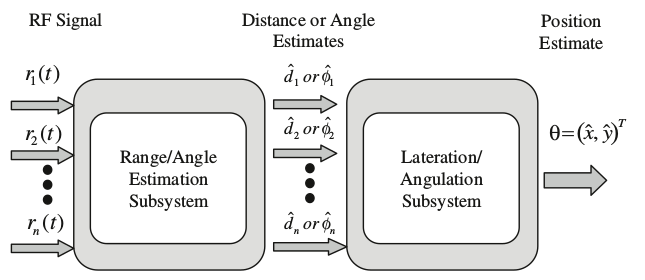
\includegraphics{figures/localization_example}
\caption{Classical geolocation system. Range or angle information is extracted from received RF signals. Location is then estimated by lateration/angulation techniques \cite{GeoLoc}.}
\label{fig:2step}
\end{figure*}



In the rest of the section we will provide an overview of the most popular ranging localization methods: TOA, TDOA, AOA, and RSS.



\subsection{Time of Arrival (TOA)}

TOA is a localization method that uses the propagation of RF signals between a mobile device and base stations of known location. The velocity of the RF signals is known, so by measuring the time that a signal takes to be received, the distance can easily be calculated. 
%The distance to at least three base stations must be calculated in order to determine the position in space.

Note that absolute times are used, so it is critical for clocks in the base stations and mobile device to be synchronized. This is not practical in many situations.

\subsection{Time Difference of Arrival (TDOA)}

\subsection{Angle of Arrival (AOA)}

\subsection{Non-Range-Based}

The previously discussed localization methods are all based on determining the distance of a receiver from RF-emitting base stations. This is not the only way localization can be done. For example, inertial tracking systems calculate position without external references. They do this using two types of sensors: accelerometers (which measure instantaneous changes in speed) and gyroscopes (which can be used to measure orientation). Using these sensors and the previous position and orientation, an updated position and orientation can be calculated. ``Dead reckoning'' is the term used to describe such a system which calculates position and orientation using differential measurements of speed and direction.

Inertial systems provide high accuracy over short periods of time, but even with very accurate sensors they are continuously accumulating error which will lead to significant drifts over larger periods of time. RF based methods on the other hand do not accumulate drift, but are susceptible to obstruction by buildings and construction materials. Therefore RF and inertial based localization methods are complementary, because the intertial method continues calculations while the RF signal is lost, and the RF method corrects for drifts over time. In the future hybrid systems are likely to become more popular as they have the potential to be more accurate and robust.

\subsection{Old}

Review of ranging and localization methods, theory behind it, application, limitations. 

TOA,
 
TDOA,

AOA ?,

non-range-based? 

"Geolocation techniques"

\cite{GeoLoc}
\cite{LiuSurvey}


\section{Contributions and Organization of the Thesis}

\subsection{Contributions  of the Thesis} \label{contributions}
single source localization

something like:

the material developed here / mathematical tools and methods are suitable for many different scenarios 
OR
can have different world life applications, for example: TOA, TDOA, static positioning using UWB range measurements. 

This work mostly investigated possible localization solution for the wireless sensor networks that use radio frequency measurements to obtain the range or range-difference measurements. However, some of the methods presented in this work can also be applied for other mediums, i.e. ultrasonic, sonic, light. 

In this paper, which considers both problems, the main focus is on efficient computation of least squares (LS) estimates of the source’s coordinate vector. The models that we consider for the said vector are based on  the assumption that the sensor network can be used, along with some form of preprocessing, to obtain (noisy) range or range-difference measurements. From a practical standpoint, this is a simplifying assumption (e.g., in nonline-of-sight scenarios), albeit one commonly made in \cite{Cheung} and \cite{classMDS} ([7] and [8]). Even so, the resulting location estimation problems are nonconvex and, therefore, rather difficult to solve globally, which explains why only approximate solutions to them have appeared in \cite{SmithAbel}, ~, \cite{LiHu} ([1], [2], [5],) and \cite{Cheung}. We should also mention here the family of data fusion methods \cite{Sayed} in which linear least squares problems are constructed via subtraction of equations. However, these methods do not provide optimal solutions since they implicitly assume the existence of an error-free measurement. In this paper, we first consider the problem of source localization from range measurements. In Section II we provide a result that explains why a recently proposed semidefinite relaxation (SDR) \cite{Cheung} of the R-LS approach to this problem may yield an accurate approximation; however, we also show that the SDR may lead to a poor approximation. For lack of a good solution to the R-LS problem, we then turn our attention to an SR-LS approach. Although the latter approach also leads to a nonconvex problem, we show that this problem can be efficiently and globally solved. Then we go on to consider the source localization problem from range-difference measurements in Section III. Our main results here concern an SRD-LS approach to this problem. In particular, we show that despite the fact that the said SRD-LS problem is also nonconvex, it can be efficiently solved, and we provide the details of an algorithm that computes the global solution of this problem. We end Section III by remarking that an SDR approach applied to a corresponding RD-LS criterion leads to extremely poor solutions. Several numerical examples suggest that the exact SR-LS and SRD-LS solutions can be more accurate by several orders of magnitude than existing approximate SR-LS and SRD-LS estimates, and than SDR-based approximations of the R-LS and
RD-LS solutions.

\subsection{Organization of the Thesis} \label{organization}

\begin{description}
\item[\textbf{Chapter 1}] contains a statement of
the claims which will be proved by this dissertation followed by an overview of the structure of the document itself. Describes in details the open problem which is to be tackled together with its context, its impact and the overall motivation for the research overall.
\item[\textbf{Chapter 2}] IRW-SR-LS.
\item[\textbf{Chapter 3}] PCCP.
\item[\textbf{Chapter 4}] Sequential Relaxation.
\item[\textbf{Chapter 6}] contains a restatement of the claims and results of the dissertation. It also enumerates avenues of future work for further development of the concept and its applications.
\end{description}